\documentclass[a4paper,12pt, titlepage]{article} 
% пакет для задания полей страницы командой \geometry :
\usepackage{geometry}
\geometry{left=3cm,right=1.5cm,top=2cm,bottom=2cm}
\usepackage[utf8]{inputenc}
\usepackage[english,russian]{babel}
\usepackage{amsmath}
%\usepackage{amsthm}
%\usepackage{cmap}
\usepackage{indentfirst}
\usepackage{a4wide,amssymb}
%\usepackage[pdftex]{graphicx}
%\usepackage[pdftex]{graphics}
%\usepackage{wrapfig}
%\linespread{1.3}               % полтора интервала. Если 1.6, то два интервала
\pagestyle{plain}               % номерует страницы

\usepackage{graphicx}
\renewcommand{\topfraction}{1}
\renewcommand{\textfraction}{0}

% The following code enables back references:
\usepackage{color} 
\definecolor{darkgreen}{rgb}{0,.5,0} 
\usepackage[unicode,colorlinks,filecolor=blue,citecolor=darkgreen,pagebackref]
{hyperref}


%opening
\title{Восстановление многогранника по набору его теневых контуров \\ Обзор
материалов и план работы}
\author{Палачев Илья}

\begin{document}

\maketitle

\tableofcontents

\section{Постановка задачи}


Имеется некоторый физический камень, геометрическая форма которого
представляет собой многогранник. Имеется установка, которая позволяет получать
информацию о его форме следующим образом:
 
\begin{enumerate}
  \item Камень жестко закрепляется одной своей гранью на горизонтальной
  подставке.
  \item Производится фотографирование камня вдоль некоторого фиксированного
  горизонтального направления $\nu_{0}$.
  \item Результатом фотографирования является монохромное изображение без
  каких-либо внутренних ребер, иными словами, "тень" камня.
  \item Затем подставка вместе с закрепленным на ней камнем поворачивается на
  фиксированный угол $\alpha_{0}$ в горизонтальной плоскости и процесс
  повторяется начиная с пункта 2.
\end{enumerate}
 
Этот процесс повторяется $K = \frac{2 \pi}{\alpha_{0}}$ раз, пока не получатся
фотографии камня по всем направлениям $\alpha_{k} = k \alpha_{0}$, где
$k = 1, 2, \ldots, K$. Все эти фотографии подвергаются обработке, в результате
которых получаются так называемые \textbf{теневые контуры} -- многоугольники,
лежащие в плоскостях, ортогональных горизонтальным векторам, образующим углы
$\alpha_{k} = k \alpha_{0}$ с осью $Ox$. 

Требуется построить трехмерный многогранник, форма которого наилучшим образом
соответствует исходному камню. При этом под качеством построенной модели
подразумевается следующее:

\begin{enumerate}
 \item Тени модельного многогранника наилучшим образом приближают тени,
 полученные из измерений.
 \item В многограннике характерные вершины и грани не разделены на несколько
 вершин и граней.
\end{enumerate}

\section{Исторический обзор смежных вопросов}

Далее приводится обзор некоторых статей, которые были написаны в целях решения
задач, схожих с рассматриваемой. Как оказалось, особенно большое сходство было
найдено с задачей оценки опорной функции в геометрической томографии. В целях
последовательности изложения сначала приводится понятие опорной функции, а
затем задачи и алгоритмы их решения.

\subsection{Понятие опорной функции выпуклого тела}

Для простоты будем рассматривать выпуклые тела в трехмерном пространстве
$\mathbb{R}^{3}$, содержащие в своей внутренности начало координат $O$.
Для некоторых понятий будем давать определения и формулировки для случая
произвольной конечной размерности.

Как известно, выпуклое тело можно однозначно представить как пересечение 
полупространств всех его касательных плоскостей 
$K = \bigcap \limits_{x \in K} R_{x}$, где $R_{x}$ -- то из двух
полупространств, на которые плоскость $\pi_{x}$, касательная к телу $K$ в
точке $x$, делит $\mathbb{R}^{3}$, которое содержит в себе целиком все тело
$K$. Всякому выпуклому телу можно поставить в соответствие набор касательных 
плоскостей $\pi_{x}$, по которым его можно построить. Обратное неверно: не
всякому произвольному набору плоскостей можно поставить в соответствие тело,
касающееся всех этих плоскостей.

Всякую касательную плоскость $\pi_{x}$ можно однозначно охарактеризовать
единичным вектором нормали $u_{x}$ и расстоянием $h_{x}$ от начала координат 
$O$ до плоскости. Поскольку две разные касательные плоскости не могут иметь
одинаковые векторы нормалей, то можно рассматривать множество всех касательных
плоскостей выпуклого тела как функцию, определенную на всех единичных векторах
$u \in S_{2}$:

$$h_{K}: S^{2} \to \mathbb{R}_{+}$$

Более общее понятие включающее в себя выше указанное было введено в 1903 году
Минковским.

\begin{flushleft}
\textbf{Определение}. Будем называть \textbf{опорной функцией} выпуклого тела
$K \subset \mathbb{R}^{n}$ следующую функцию 
$h_{K}: \mathbb{R}^{n} \to \mathbb{R}_{+}$:

$$h_{K}(u) = \max \limits_{x \in K}(x, u)$$
\end{flushleft}

Если взять некоторую точку $u_{0}$ на единичной сфере $S^{n - 1}$, и вычислить
в ней значение опорной функции $h_{K}(u_{0})$, то по этим данным можно
построить касательную плоскость к выпуклому телу в некоторой (неизвестной!)
точке $x \in K$. Такую плоскость (в контексте, когда нет информации о положении
точки касания) принято называть опорной плоскостью.

\begin{flushleft}
 \textbf{Определение}. \textbf{Опорной плоскотью} выпуклого тела $K$ по
 направлению $u \in S^{n - 1}$ называется плоскость с нормалью $u$, расстояние
 от которой до начала координат равно $h_{K}(u)$
\end{flushleft}

Очевидно, что опорная функция выпуклого тела обладает следующим свойством:

$$h_{K}(\lambda u) = \lambda h_{K}(u)$$

Следовательно, для практики достаточно иметь дело только с ограничением опорной
функции на единичную сферу. В статье \cite{journals/jmiv/KarlKVW96} вводится
понятие \textbf{приведенной опорной функции}:

$$H_{K} (u) = h_{K} (\frac{u}{||u||})$$

которая в действительности педставляет собой расстояние от начала координат
$\mathbb{O}$ до опорной гиперплоскости по направлению $u$.

Более подробно свойства опрной функции рассматриваются в статье
\cite{journals/cviu/GhoshK98}.

%(TODO: прочесть и законспектировать)

\subsection{Восстановление выпуклого многоугольника по измерениям его опорной
функции (по статье Prince, Willsky)}

В работе \cite[Prince - Willsky (1990)]{journals/pami/PrinceW90}
рассматриваются алгоритмы для восстановления \textbf{двумерных} выпуклых тел по
измерениям их опорных функций. Изначально изучение данной проблемы было
мотивировано задачей из компьютерной томографии. А именно, в томографии
делаются измерения интегралов плотности поглощения излучения объектом вдоль
различных фиксированных прямых. Допустим, что известны интегралы плотности
поглощения по пучку прямых $L(t, \theta)$, где угол $\theta$ фиксирован. Тогда
по этой информации можно определить положение двух опорных прямых к данному
объекту (см. рис. \ref{tomography-application}).

\begin{figure}[ht]
    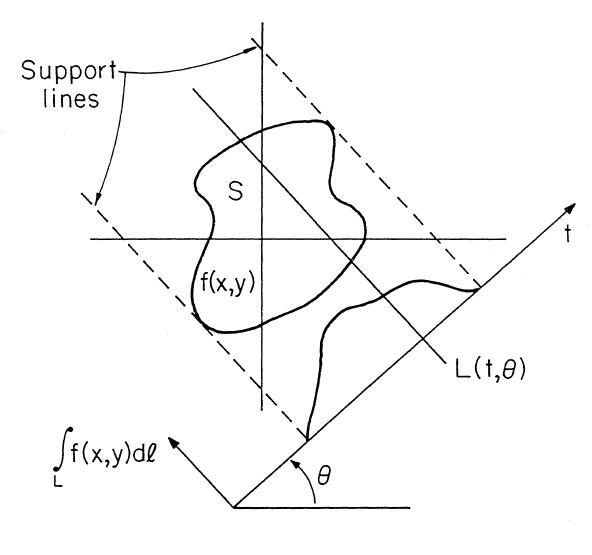
\includegraphics[width=10cm]{images/tomography-application.jpg}
    \caption{Граница носителя функции плотности поглощения определяет две
    опорные прямые к объекту}
    \label{tomography-application}
\end{figure}

По имеющимся измерениям опорной функции можно потроить грубое приближение
расмматриваемого тела -- путем обыкновенного пересечения полуплоскостей,
соответствующих опорным прямым. Однако на практике измерения подвержены
ошибкам и известны лишь с некоторой точностью. Так, может оказаться, что
после пересечения построенное тело будет касаться не всех заданных прямых.
Это приводит к тому, что всего одно грубое измеренние может заблокировать
воздействие других (более точных) измерений на результат (см. рис.
\ref{inconsistent}).

\begin{figure}[ht]
    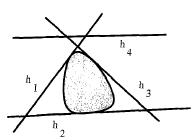
\includegraphics[width=10cm]{images/inconsistent-support-planes.jpg}
    \caption{В случае неточных измерений опорной функции тело нельзя строить
    как пересечение полупространств}
    \label{inconsistent}
\end{figure}

Prince и Willsky рассматривают в своей статье случай, когда измерения опорной
функции получаются по фиксированному набору направлений

$$u_{i} = (cos \theta_{i}, sin \theta_{i})$$

где углы $\theta_{i}$ берутся по всему отрезку $[0, 2 \pi]$ с постоянным шагом:

$$\theta_{i} = i \cdot \Delta \theta$$

где $\Delta \theta = \frac{2 \pi}{M}, i = 0, \ldots, M - 1, M \leq 5$. Более
общий случай, когда направления измерений выбираются произвольным образом,
описывается в статье
\cite[Lele - Kulkarni - Willsky (1992)]{journals/josaa/LeleKW92}.

Ключевым понятием в статье является следующее

\begin{flushleft}
 \textbf{Определение}. \textbf{Набором опорных чисел}
 $(h_{0}, h_{1}, \ldots, h_{M - 1})^{T}$выпуклого тела $K$ по заданному набору
 направлений $u_{i}, i = 0, \ldots, M - 1$ называется называется вектор в
 $\mathbb{R}^{M}$, составленный из значений опорной функции по соответствующим
 направлениям: $(h_{K}(u_{0}), h_{K}(u_{1}), \ldots, h_{K}(u_{M - 1}))^{T}$.
\end{flushleft}

Основным теоретическим результатом статьи, на котором основаны все алгоритмы,
является следующая

\begin{flushleft}
 \textbf{Теорема 1}. \textbf{Опорная теорема}

  Набор действительных чисел $h \in \mathbb{R}^{M}, M \leq 5$ является набором
  опорных чисел тогда и только тогда, когда
  
  $$h^{T} C \leq (0, \ldots, 0)$$
  
  где $C$ -- $M \times M$ матрица, заданная следующим образом:
  
  $$
  C = 
  \left(
  \begin{array}{ccccccc}
       1 &     -k &      0 & \ldots &      0 &      0 &     -k \\
      -k &      1 &     -k & \ldots &      0 &      0 &      0 \\
       0 &     -k &      1 & \ldots &      0 &      0 &      0 \\
  \vdots & \vdots & \vdots & \ddots & \vdots & \vdots & \vdots \\
       0 &      0 &      0 & \ldots &      1 &     -k &      0 \\
       0 &      0 &      0 & \ldots &     -k &      1 &     -k \\
      -k &      0 &      0 & \ldots &      0 &     -k &      1 \\
 \end{array}
 \right)
  $$
  
  где $k = 1 / (2 cos(\frac{2 \pi}{M}))$.

\end{flushleft}

Таким образом, все возможные наборы $h \in \mathbb{R}^{M}$ образуют конус в
$\mathbb{R}^{M}$.

\begin{flushleft}
 \textbf{Определение}. \textbf{Опорным конусом} размерности $M$ называется
 множество:
 $$
 \mathfrak{C} = \{h \in \mathbb{R}^{M} | h^{T} C \leq (0 \ldots 0) \}
 $$
\end{flushleft}

Дальнейшая часть статьи посвящена, собственно, нахождению такой точки 
$h \in \mathbb{R}^{M}$ в
опорном конусе (т. е. такого набора чисел, который является набором опорных
чисел), который бы соответствовал следующим критериям:

\begin{enumerate}
 \item Расстояние от $h$ до вектора $y \in \mathbb{R}^{M}$, полученного из
измерений, минимально
 \item Потроенное по набору опорных чисел выпуклое тело соответствует
известной априорной информации об объекте.
\end{enumerate}

Под априорной информаций во втором пункте подразумевается, например, известное
положение центра масс вершин полученного многоугольника, или тот факт, что
поверхность тела обладает гладкостью (далее это понятие будет разъяснено).

Прежде всего в статье приводится детальный анализ опорного конуса $\mathfrak{C}$
-- множества, на котором производится минимизация функционала. Поскольку матрица
$C$ циклическая, ее собственные числа можно получить при помощи дискретного
преобразования Фурье ее первой строки (TODO: обосновать). А именно, они равны

$$
\lambda_{k} = 1 - \frac{cos(2 \pi (k - 1) / M)}{cos(2 \pi / M)},
k = 1, \ldots, M
$$

Очевидно, что ровно два собственных значения являются нулевыми:
$\lambda_{2} = \lambda_{M} = 1 - \frac{cos(2 \pi / M)}{cos(2 \pi / M)} = 0$.
Следовательно, матрица $C$ является сингулярной и ее ядро $\mathfrak{N}$ есть
двумерное подпространство, имеющее следующие базисные векторы:

$$
n_{1} = (1, cos(\theta_{0}), cos(2 \theta_{0}), \ldots,
cos((M - 1) \theta_{0}))^{T}
$$

$$
n_{2} = (0, sin(\theta_{0}), sin(2 \theta_{0}), \ldots,
sin((M - 1) \theta_{0}))^{T}
$$

где $\theta_{0} = 2 \pi / M$.

Геометрическим следствием этого факта является то, что конус $\mathfrak{C}$ не
является правильным конусом, поскольку целиком сожержит в себе линейное
подпространство размерности 2. Следовательно, опорный конус является декартвым
произведением правильного конуса
$\mathfrak{C}_{p} = {h \in \mathfrak{C} | h^{T} n_{1} = 0, h^{T} n_{2} = 0}$
и ядра $\mathfrak{N}$ матрицы $C$. Соответственно, любой вектор, составленный из
набора опорных чисел, является покомпонентной суммой ортогональных векторов
$h_{p} \in \mathfrak{C}_{p}$ и $h_{n} \in \mathfrak{N}$:

$$h = h_{p} + h_{n}$$

Далее в статье показано, что компонента $h_{n}$ есть по сути плоскопараллельный
сдвиг вектора $h$, составленного из набора опорных чисел в пространстве
$\mathbb{R}^{2}$.

Пусть имеется некоторый фиксированный (согласованный) вектор $h$, составленный
из набора опорных чисел. Тогда существует, вообще говоря, целое семейство
выпуклых множеств на плоскости $\mathbb{R}^{2}$, для которых вектор $h$ является
вектором опорных чисел. Наибольшее из из этих множеств $S_{B}$ определяется как
пересечение полупространств, образованных опорными прямыми:

$$
S_{B} = \{u \in \mathbb{R}^{2} |
u^{T} (\omega_{1} \omega_{2} \ldots \omega_{M}) \leq
(h_{1} h_{2} \ldots h_{M})\}
$$


\section{Предлагаемый подход}

\newpage
\bibliographystyle{plain}
\bibliography{references}

\end{document}
